\section{IR of Industrial Compilers}
\frame{
\frametitle{IR of Industrial Compilers :: LLVM Bitcode \\
Local variables handled \textit{differently} in IR and ASM
}
\begin{columns}
\begin{column}{0.70\textwidth}
    \begin{center}
     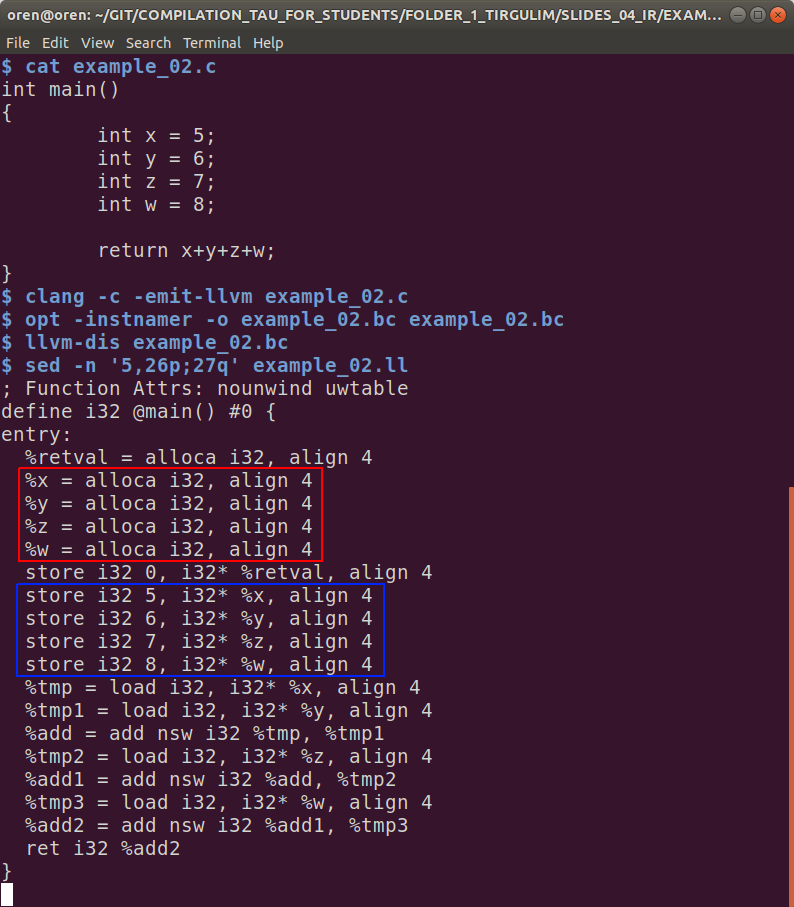
\includegraphics[width=0.75\textwidth]{example_02.png}
     \end{center}
\end{column}
\begin{column}{0.5\textwidth}
\begin{itemize}
\item
allocations ({\color{red} red})
\begin{itemize}
\item
on main's stack frame
\item
no default value
\end{itemize}
\item
stores ({\color{blue} blue})
\begin{itemize}
\item
name based access
\item
should eventually be \\
translated to some relative
offset from the frame pointer
\end{itemize}
\item
loads (how many?)
\begin{itemize}
\item
name based access
\item
should eventually be \\
translated to some relative
offset from the frame pointer
\end{itemize}
\end{itemize}
\end{column}
\end{columns}
}